% Nejprve uvedeme tridu dokumentu s volbami
\documentclass[czech,master,public,dept460,male,cpdeclaration,oneside]{diploma}

\usepackage[autostyle=true,czech=quotes]{csquotes} % korektni sazba uvozovek, podpora pro balik biblatex
\usepackage{subfig}		% makra pro "podobrazky" a "podtabulky"
\usepackage{tikz}		% makra pro kresleni
\usepackage{cite}
\usepackage[thinlines]{easytable}
\usepackage{graphicx}
\usepackage{vcell}

%\usepackage[backend=biber, style=iso-numeric, alldates=iso]{biblatex} % bibliografie
\usepackage{dcolumn} % sloupce tabulky s ciselnymi hodnotami
\usepackage{subfig} % makra pro "podobrazky" a "podtabulky"

% Zadame pozadovane vstupy pro generovani titulnich stran.
\ThesisAuthor{Bc. Lukáš Stankovič}

\CzechThesisTitle{Kvalita a měření softwarových procesů}

\EnglishThesisTitle{Software Process Quality and Measurement}

\SubmissionDate{20. dubna 2021}

\Thanks{TODO}

% Zadame cestu a jmeno souboru ci nekolika souboru s digitalizovanou podobou zadani prace.
% Pokud toto makro zapoznamkujeme sazi se stranka s upozornenim.
\ThesisAssignmentImagePath{Diplomka/Figures/Assignment}

% Zadame soubor s digitalizovanou podobou prohlaseni autora zaverecne prace.
% Pokud toto makro zapoznamkujeme sazi se cisty text prohlaseni.
\AuthorDeclarationImageFile{Diplomka/Figures/AuthorDeclaration.jpg}

% Zadame soubor s digitalizovanou podobou souhlasu spolupracujici prav. nebo fyz. osoby.
% Pokud toto makro zapoznamkujeme sazi se cisty text souhlasu.
\CooperatingPersonsDeclarationImageFile{Diplomka/Figures/CoopPersonDeclaration.jpg}

\CzechAbstract{}

\CzechKeywords{}

\EnglishAbstract{}

\EnglishKeywords{}

\AddAcronym{ALM}{Application lifecycle anagement}
\AddAcronym{Automotive SPICE}{Automotive Software Process Improvement and Capability Determination}
\AddAcronym{SIG}{Automotive Special Interest Group}
\AddAcronym{VDA QMC}{Quality Management Center in the German Association of Automotive Industry}
\AddAcronym{RUP}{Rational Unified Process}
\AddAcronym{BIRT}{Business Intelligence and Reporting Tools}
\AddAcronym{IDE}{Integrated Development Environment}
\AddAcronym{SVG}{Scalable Vector Graphics}
\AddAcronym{JDBC}{Java Database Connectivity}
\AddAcronym{XML}{Extensible Markup Language}
\AddAcronym{ODA}{Open Data Access}
\AddAcronym{SEI}{Software Engineering Institute}
\AddAcronym{CMM}{Capability Maturity Model}
% \addbibresource{biblatex-examples.bib}
% \addbibresource{coffee.bib}

% Novy druh tabulkoveho sloupce, ve kterem jsou cisla zarovnana podle desetinne carky
\newcolumntype{d}[1]{D{,}{,}{#1}}


% Zacatek dokumentu
\begin{document}

% Nechame vysazet titulni strany.
\MakeTitlePages

 \lstlistoflistings
 
% A nasleduje text zaverecne prace.
\section{Úvod}
\label{sec:Introduction}

Při vývoji téměř jakéhokoli nejen softwarového produktu je potřeba se věnovat vývojovému procesu. Vývojový proces slouží k tomu, aby byl daný produkt vyvinut v určitých kvalitách a řízen správným směrem. Softwarový proces kromě standardizace řízení a plánování definuje také jednotlivé kroky k vytvoření softwarového produktu. [CT]. Vyvíjet s daným softwarovým procesem nám může zaručit, že produkt jež je vytvářen bude kvalitní a bude dokončen v definovaném termínu. 

Během každého softwarového procesu je nutné jednotlivé kroky plánovat, monitorovat a na základě získaných dat vývoj uzpůsobovat. Monitorování procesu probíhá pomocí metrik, které mohou být reprezentovány buď pomocí tabulky nebo vizualizovány pomocí grafu. Veškeré sledování a měření daného procesu by bylo bez pomocných nástrojů velmi složité. Proto existuje nespočet nástrojů a aplikací, které v řízení pomůžou. Těmto aplikacím se dále v práci věnuji. V práci se zaměřuji především na metriky sběru požadavků.

Práce je rozdělena na teoretickou a praktickou část. V teoretické části se věnuji softwarovému inženýrství, softwarovým procesům a samotnému vývoji nejen softwaru, ale také v automobilovém vývoji pomocí standardu Automotive SPICE. V práci se také věnuji jednotlivým typů procesu jako je vodopádový model nebo agilní přístupy. Dále rozebírám jednotlivé metriky a možnosti použití v různých procesech.

Cílem praktické části práce je analyzovat nástroje pro správu nasbíraných požadavků a jejich následnou vizualizaci pomocí metrik. V rámci práce jsem vypracoval vlastní aplikaci sloužící pro agregaci dat z IBM Jazz, které verzuji a následně vizualizuji pomocí uživatelsky definovaných metrik. Velkou výhodou je univerzálnost aplikace na zvoleném softwarovém procesu. Během vývoje aplikace jsem si vyzkoušel jednotlivé fáze vývoje. Věnoval jsem se například analýze požadavků a vytvořil jsem případy užití. Také jsem si pro jednotlivé části aplikace navrhl uživatelské rozhraní pomocí drátových modelů.


\textbf{bude dopsáno + citace}

\section{Softwarový proces}
\label{sec:sw_process}

Dle Iana Sommervilla \cite{ref:sommerrville_sw_process} je softwarový proces sekvence souvisejících aktivit, které vedou k produkci softwarovécho produktu. Tyto aktivity mohou probíhat buď v rámci vývoj softwarového produkt od nuly nebo úpravě již existujícího softwarového produktu. Existuje nespočet různých softwarových procesů. Všechny softwarové procesy by měly obsahovat následující čtyři aktivity:

\begin{enumerate}
\item \textit{Specifikace} -- během této aktivity je nutné zjistit a definovat požadavky zákazníka na budoucí software.
\item \textit{Návrh a implementace softwaru} -- na základě specifikovaných zákaznických požadavků je software navrhnut a poté implementován.
\item \textit{Validace softwaru }-- je nutné software validovat, aby bylo zajištěno, že jeho funkcionalita odpovídá předem specifikovaným požadavkům.
\item \textit{Evoluce softwaru} -- software se během používání mění, aby vyhovoval novým potřebám zákazníka.
\end{enumerate}

Softwarové procesy je nutné vždy používat na základě vyvíjeného produktu. V praxi neexistuje žádný softwarový proces, který by pokrýval a řešil veškeré problémy při vývoji softwaru. Pro zjednodušení softwarového procesu slouží různé softwarové modely. Ty se dělí na plánované, inkrementální a agilní. Při vývoji velkého systému se můžou jednotlivé modely softwarových procesů kombinovat. Vyspělost společnosti v používání softwarových procesů můžeme hodnotit podle stupnice SEI (Software
Engineering Institute). Model hodnocení vyspělosti používání softwarového procesu dané společnosti se nazývá CMM (Capability Maturity Model), přičemž můžeme společnost hodnotit od 1 do 5 \cite{ref:sw_process_vondrak}:

\begin{enumerate}
\item \textit{Počáteční} -- společnost nepoužívá žádný softwarový proces. Jelikož žádný softwarový proces není definován tak každý projekt je vyvíjen případ od případu.
\item \textit{Opakovatelná} -- sledovaná společnost identifikovala ve svých projektech postupy, které se často opakují. Tyto prováděné opakované činnosti poté systémově opakuje v každém novém projektu.
\item \textit{Definovaná} -- používaný softwarový proces je definovaná a dokumentován na základě vysledovaných opakovatelných kroků.
\item \textit{Řízená} -- jakmile má daná společnost definovaný a dokumentovaný softwarový proces, je společnost schopna daný proces řídit a monitorovat. 
\item \textit{Optimalizovaná} -- na základě dlouhodobě vysledovaných dat při používání softwarového procesu je společnost schopná daný softwarový proces optimalizovat a vylepšit tak, aby více vyhovoval celému vývoji.
\end{enumerate}


\subsection{Plánování}
Je to jedna z částí softwarového procesu. Velikost a důkladnost plánování procesu a samotného projektu závisí na používaném modelu softwarového procesu. Například při použití vodopádového modelu je plánování velmi důležitá část procesu, jelikož na kvalitní specifikaci a plánování kompletního procesu stojí celý vývoj. Naopak při vývoji pomocí agilních způsobů je část plánování a specifikace softwaru minimální. 

Během plánování probíhá kromě plánování samotného procesu také specifikace výsledného softwaru. Specifikace vyvíjeného softwaru je část procesu, během které dokážeme určit a definovat, které vlastnosti budou od systému požadovány. Vlastnosti a požadavky na systém vzniknou sběrem požadavků od zákazníka, který má na vznikající software určité nároky. Tento proces bývá také nazýván inženýring požadavků. Bývá jednou z nejkritičtějších částí, jelikož chybná specifikace jednotlivých požadavků v této fázi vedou k pozdějším problémům jak při samotném návrhu a implementaci, tak i při pozdější správě.

Cílem inženýringu požadavků je získat od zákazníka co nejvíce požadavků, které na budoucí software klade. Na základě nasbíraných požadavků vznikne dokument schválených požadavků pro  implementaci a následnou dokumentaci celého softwaru. Dále na základě získaných požadavků je vytvořen plán celého vývoje softwaru. U vodopádového modelu inženýring požadavků probíhá na začátku vývoje a je velmi detailní. Při agilních a iterativních způsobech vývoje probíhá sběr požadavků vždy před každou iterací.

\subsection{Monitorování}
Další důležitou částí každého softwarového procesu je jeho monitorování. Během monitorování zjišťujeme, zda proces probíhá tak jak jsme ho plánovali a také, zda neexistují možnosti, jak proces zlepšit a tím dosáhnout lepších výsledků. Monitorování je nepřetržitý proces, který také kromě zlepšování procesu zahrnuje sledování, aby bylo možné identifikovat potenciální problémy dostatečně včas, než způsobí závažný problém. Samotné monitorování je často prováděno současně s kontrolou a uzpůsobením daného procesu (viz kapitola \ref{sec:control}).

Hlavním důvodem pro monitorování procesu je, že výkonnost a daného procesu je důkladně sledován. Díky tomu je možné rychle identifikovat odchylky od původního plánovaného plánu daného projektu. Během monitorování také sledujeme, zda se plní nadefinované požadavky a jak rychle. K tomuto účelu mohou sloužit metriky (viz kapitola \ref{sec:metrics}).

Obecně lze monitorovat tři typy metrik určitého procesu:

\begin{enumerate}
\item \textit{Čas potřebný k dokončení určitého procesu} -- můžeme zde zařadit například celkový čas strávený na úkolech a požadavcích potřebných k dokončení vývoje, čas strávený testováním a další.

\item \textit{Prostředky potřebné pro určitý proces} -- řadíme zde různé prostředky, které jsou nutné pro úspěšné dokončení procesu. Jde například o cestovní náklady pro manažera, výpočetní zdroje a další.

\item \textit{Počet výskytů nějaké definované události} -- v rámci tohoto typu můžeme zařadit například počty nalezených chyb, počet zbývajících nedokončených úkolů, počet schválených požadavků, celkový počet požadavků a mnoho dalšího.
\end{enumerate}

Monitorování procesu představuje způsob, pomocí kterého můžeme vytvářet doklady o daném procesu a jeho změnách. Pomocí monitorování dokážeme určit, zda je proces efektivní a zda případné změny procesu mají na proces pozitivní dopad. Pro správnou interpretaci změn by mělo být měření pouhou částí. Abychom si byli jisti správnostmi změn procesu, musíme měření kombinovat s kvalitativním hodnocením změn a správnou komunikací o zavedených změnách s účastníky procesu. Díky správné komunikaci dokážeme zjistit jejich názory na efektivitu provedených změn procesu a dokážeme odhalit další faktory, které by mohly proces negativně ovlivnit. Pomocí monitorování chování týmu po zavedené změně dokážeme pozorovat jak daný tým změny přijal a jaká panuje v týmu nálada.

\subsection{Uzpůsobení}
\label{sec:control}
Proces bychom měli pravidelně uzpůsobovat potřebám, které se mohou v rámci vývoje produktu měnit. Podměty ke změnám daného softwarového procesu získáváme z monitorování procesu. V rámci uzpůsobení řešíme také, zda je projekt stihnutelný v definovaném termínu. Tuto informaci nejčastěji zjistíme pomocí vytvořených metrik.

Samotné uzpůsobení procesu může probíhat několikrát během celého vývoje. Během uzpůsobení také provádíme validaci celého procesu a řešíme, zda není možné někde dělat nějakou část lépe a efektivněji. V rámci uzpůsobení se také validuje, zda v daném procesu postupujeme správně a zda probíhá vše tak, jak bylo v rámci procesu definováno. V rámci uzpůsobení a zlepšování procesu můžeme použít několik konceptů.

Uzpůsobení procesu může být kromě úprav existujícího procesu provedeno jako vytvoření úplně nového procesu nebo nahrazení starého procesu jiným. Dále můžeme proces uzpůsobit zavedením nového nástroje, změnou metod, zavedením nových rolí nebo také pouhou změnou komunikace. Po jakékoli změně a uzpůsobení procesu je nutné pozorovat a měřit pomocí metrik, zda byla změna vhodná a prospěšná. Obecně není rozumné zavádět více změň v jednu dobu, jelikož poté není jednoduché změřit, zda změna byla prospěšná či nikoli.

\subsubsection{CMM a CMMI}
CMM je vývojový model, který byl vyvinut institutem SEI v 80. letech 20. století. Vznikl jako výsledek studie při níž byla sesbírána data různých organizací a byla financovaná ministerstvem obrany Spojených států amerických. Je to systém pravidel a cílů pro zlepšení práce a procesů. Model CMM také obsahuje model zralosti lidských schopností a model možností systémového inženýrství. Model byl primárně vytvořen pro vývoj softwaru, ale je možné jej použít prakticky skoro při jakémkoli vývoji nového produktu. \cite{ref:cmm_cmmi}

Automotive SPICE používá pro hodnocení, úpravu a zlepšování procesů vlastní systém, který je však vytvořen právě z CMM. Konkrétně z modelu CMM standard využívá úrovně zralosti SEI. Model je však rozšířen o základní model procesů. Ten je například používán jako výchozí bod při definování konkrétních procesů. Tento přístup vychází z obecného standardu SPICE, který je používán mimo automobilový průmysl.

Z tohoto modelu vychází novější vývojový model CMMI, který slouží primárně jako architektura pro následné zlepšení procesů v jakékoli organizaci. Stejně jako vývojový model SPICE obsahuje úrovně způsobilosti, které hodnotí vyškolený hodnotitel. Úrovně způsobilosti jsou definovány jako škála 0 až 5, přičemž je možné hodnotit desítky oblastí procesu. Na základě tohoto hodnocení mohou poté probíhat úpravy a vylepšování používaného procesu nebo zavedení úplně nových procesů. Veškeré cíle a postupy, které jsou doporučovány a upravovány v rámci procesu jsou obecné a nejsou tedy technicky zaměřené.

\subsubsection{PDCA}
Je to iterativní metoda, jejíž cílem je dosáhnout stálého zdokonalování procesů, zvýšení kvality výsledného systému, zlepšení služeb a další. Metoda je založena na čtyřech základních krocích, které se pravidelně opakují. Existuje také varianta s pěti kroky nazývána OPDCA. Metodu PDCA je možné použít prakticky ve všech oborech, kde se vyvíjí nějaký systém, nebo produkt.  Jednotlivé kroky metody PDCA jsou následující:

\begin{enumerate}
\item \textit{Naplánuj} -- Během prvního kroku se na základě stávajících podmínek a procesů naplánuje a definují nezbytné kroky pro následující změnu. Nezbytnou součástí každého plánu musí být konkrétní způsoby, jak změny realizovat. Další důležitým bodem, který musí být promyšlen je zajištění zdrojů pro provedení dané změny.
\item \textit{Proveď} -- V rámci tohoto koku je prováděna realizace naplánovaných a navržených úprav z prvního kroku. Důležité je také v tomto kroku provést dokumentaci všech změn, které byly provedeny. Během tohoto kroku se provádí měření všech provedených změn pro následnou analýzu.
\item \textit{Ověř} -- Tento krok je důležitý pro kontrolu provedených změn. Kontrola probíhá pomocí analýzy nasbíraných dat během druhého kroku. Velmi důležité je zjistit, zda se po provedených změnách proces zlepšil, nebo ne a změny byly negativního rázu. Pro vizualizaci a porovnání naměřených dat můžeme použít například grafy. Veškeré zjištěné informace se následně využijí v následujícím kroku.
\item \textit{Jednej} -- Poslední krok je založen na logickém postupu, kdy pokud bylo v předchozím kroku ověření prokázáno, že provedené změny pozitivně přispěly ke zdokonalení procesu, pak se tento upravený proces stává standardem, kterým se bude nově společnost řídit. Pokud se ukáže, že provedené změny mají negativní nebo neutrální přínos, tak se proces nezmění a společnost se řídí starým neupraveným procesem. Může se také stát, že změny přinesou nějaký neočekávaný výsledek, se kterým se v prvním plánovacím kroku nepočítalo. V takovém případě, i když mají změny pozitivní vliv, není změna přijata, ale je zahrnuta do nového cyklu a podrobně znova prozkoumána.
\end{enumerate}


\subsection{Sekvenční a iterativní přístupy vývoje}
\subsubsection{Vodopádový model}
Jde o jeden z nejstarších vývojových procesů, který byl poprvé publikován v článku v roce 1970 Winstonem W. Roycem a vychází z obecných vývojových procesů. Vodopádovým modelem je nazýván, protože jednotlivé fáze procesu postupně kaskádovitě navazují na sebe a celý model poté vypadá jako vodopád. Veškeré kroky musí být pečlivě analyzovány a naplánovány. K další vývojové fázi se přistupuje až poté, co jsou veškeré předchozí kroky splněny, schváleny a uzavřeny. \cite{ref:sommerrville_waterfall} Aby byl projekt podle modelu úspěšný je nutné věnovat prvním fázím dostatek času. Vodopádový model je možné vidět na obrázku \ref{fig:waterfall}.

\begin{figure}[!ht]
    \centering
    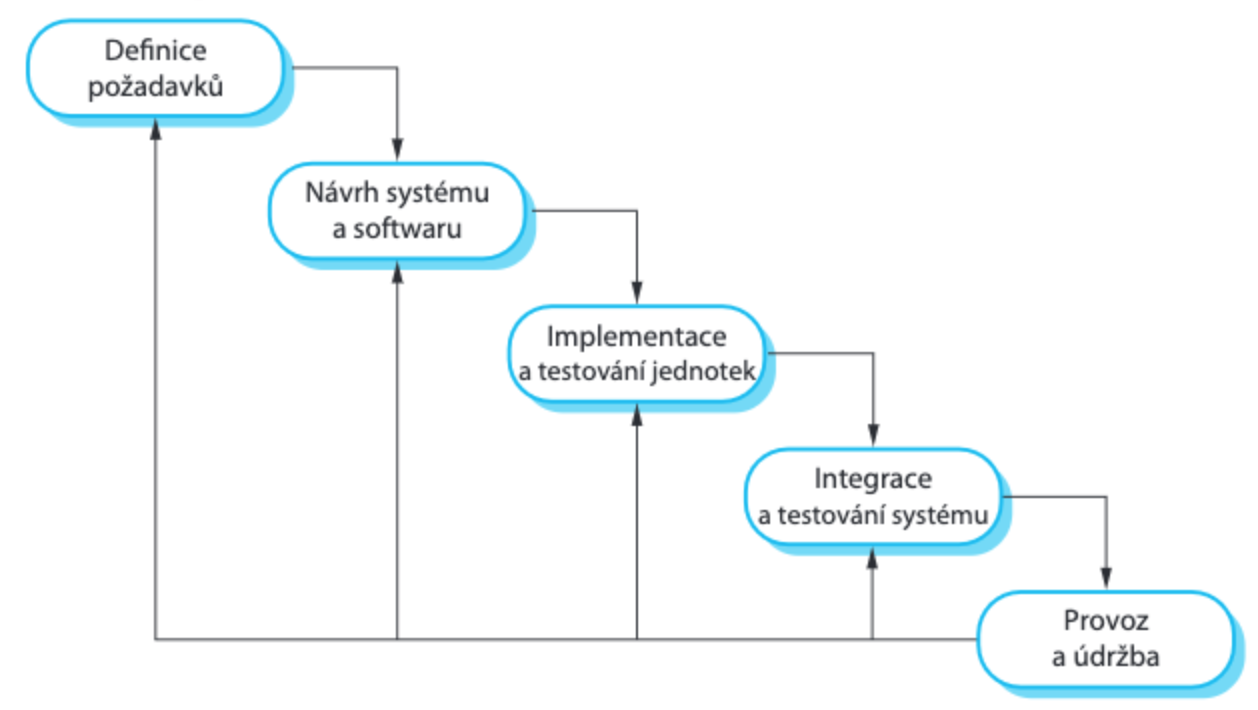
\includegraphics[width=1\textwidth]{Diplomka/Figures/waterfall.png}
    \caption{Vodopádový model (převzato z \cite{ref:sommerrville_waterfall})}
    \label{fig:waterfall}
\end{figure}

Základní fáze vodopádového modelu vychází ze standardních potřeb vývoje softwaru:

\begin{enumerate}
\item \textit{Specifikace požadavků} -- na základě jednotlivých požadavků zákazníka jsou požadavky detailně sepsány a analyzovány.

\item \textit{Systémový a softwarový návrh} -- jednotlivé požadavky zákazníka určují náročnost na systém. Návrh zahrnuje také celkovou architekturu systému. 

\item \textit{Implementace a unit testování} -- v rámci této fáze se systém realizuje a každá jednotka je samostatně testována, zda splňuje určité požadavky.

\item \textit{Integrace a testování systému} -- jednotlivé vyvinuté části systému se integrují a otestují jako kompletní systém. Tímto je zajištěno, že celý systém splňuje definované požadavky. Jakmile je produkt kompletně otestován, je předán zákazníkovi.

\item \textit{Provoz a údržba} -- během této fáze se systém nasazuje do ostrého prostředí. Během fáze probíhá oprava chyb a vylepšování funkcí.

\end{enumerate}

V praxi je složité jednotlivé fáze pečlivě oddělit a postupovat v další fáze pouze jakmile je předchozí fáze plně dokončena. Proto se většinou jednotlivé fáze postupně překrývají a vyměňují si mezi sebou informace. Hlavní nevýhoda modelu je praktická nemožnost reagovat na měnící se požadavky zákazníka. Vodopádový model je vhodné zpravidla použít tam, kde víme, že se požadavky zásadně nebudou měnit.

\subsubsection{Rational Unified Process}
Rational Unified Process (RUP) je iterativní model vývoje softwaru vytvořený firmou Rational Software Corporation. RUP byl vytvořen a odvozen z osvědčených praktik při vývoji softwaru. Mezi tyto praktiky například patří řízení změn, komponentová architektura, aktivní správa požadavků nebo například ověřování kvality software. Model obsahuje čtyři fáze, které se iterují dle potřeby. Jednotlivé fáze oproti vodopádovému modelu nesouvisejí s technickými hledisky ale spíše se soustředí na podniková hlediska. \cite{ref:rup_ibm_about} Fáze jsou následující:

\begin{enumerate}
\item \textit{Zahájení} -- cíl této fáze je vytvořit podnikový případ systému. V rámci této fáze je potřeba identifikovat veškeré osoby a další systémy které budou s daným systémem pracovat či komunikovat.
\item \textit{Příprava} -- během této fáze se vytvoří architektura systému. Dále se vytvoří celkový plán projektu a identifikují se klíčová rizika, která mohou na projektu nastat. Během fáze vznikne například plán vývoje, UML diagramy nebo popis systému.
\item \textit{Konstrukce} -- tato fáze obsahuje návrh systému, samotné programování a testování, přičemž se zároveň jednotlivé části systému integrují. Dále během této fáze vzniká dokumentace. Na konci fáze je hotový funkční produkt připravený na dodání zákazníkovi.
\item \textit{Předávání} -- v závěrečné fázi je funkční produkt spolu s dokumentací předán zákazníkovi. Produkt je nasazen do ostrého prostředí a zprovozněn.
\end{enumerate}

U modelu RUP je možné provádět inkrementaci jednak samostatným opakováním jednotlivých fází ale i celého procesu. Kromě čtyřech fází RUP definuje jednotlivé disciplíny, které jsou v rámci fázích prováděny. Velkou výhodou je, že tyto disciplíny nejsou navázány na jednotlivé fáze. Disciplíny jsou činnosti, prováděné během celého vývoje produktu. Disciplíny jsou následující:

\begin{itemize}
\item Tvorba modelu
\item Správa požadavků
\item Analýza a návrh
\item Implementace
\item Testování
\item Nasazení
\item Správa konfigurace a změn
\item Řízení projektu
\item Správa prostředí 
\end{itemize}

Výše popsané fáze společně s disciplínami je možné vidět na obrázku \ref{fig:rup}. Vidíme, že různé disciplíny mají v jednotlivých fázích vyšší důležitost než jiné.

\begin{figure}[!ht]
    \centering
    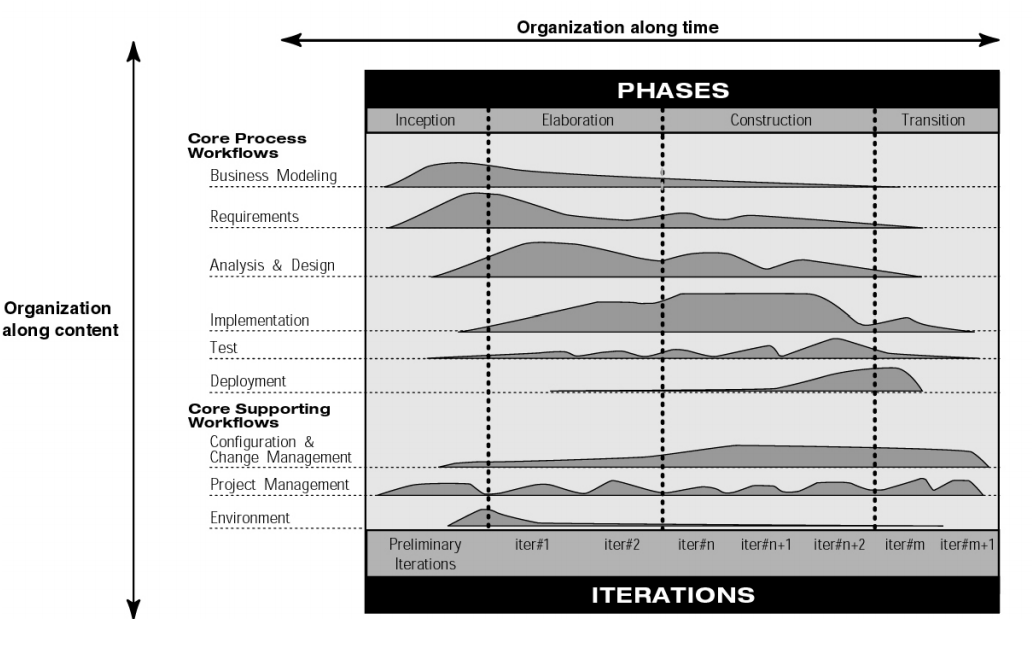
\includegraphics[width=0.75\textwidth]{Diplomka/Figures/rup.png}
    \caption{Grafické znázornění fází a disciplín RUP (převzato z \cite{ref:rup_ibm})}
    \label{fig:rup}
\end{figure}

\subsection{Agilní přístupy vývoje}
Aktuální trh se softwarem se rychle mění a proto je potřeba reagovat na měnící se prostředí. Agilní přístupy patří k inkrementálním způsobům vývoje. Software vytvářený pomocí vodopádového modelu může být v době vydání již velmi zastaralý. Z tohoto důvodu jsou agilní přístupy vývoje v poslední době velmi oblíbené. Takto vyvíjený software je většinou dodán rychleji, ale za to může být dodán s horší kvalitou. Takový přístup se ovšem nehodí u kritických systémů, u kterých je kladen velký důraz například na bezpečnost a spolehlivost. Software se během agilního vývoje vytváří ve verzích, kdy každá nová verze obsahuje nové funkcionality. Jednotlivé vývojové procesy se prolínají a většinou neexistuje podrobná specifikace a dokumentace systému. V dokumentaci obvykle bývají pouze základní a nejdůležitější prvky systému. Tento nedostatek se může ovšem rychle vymstít při následné údržbě daného softwaru.

Filozofie agilních metodik vychází z manifestu, na kterém se shodli vývojáři těchto vývojových metod. Manifest popisuje čtyři základní hodnoty, kterých si autoři cení \cite{ref:agilne_manifesto}:

\begin{itemize}
\item Jednotlivci a interakce před procesy a nástroji.
\item Fungující software před vyčerpávající dokumentací.
\item Spolupráce se zákazníkem před vyjednáváním o smlouvě.
\item Reagování na změny před dodržováním plánu.
\end{itemize}

Každý vývojový proces má svá pozitiva a svá negativa. Mezi pozitiva při agilním vývoji patří například rychlejší vývoj, větší flexibilita vývoje, kdy je možné upravovat směr dalšího vývoje dle potřeby zákazníka nebo například zapojení zákazníka do procesu vývoje. Mezi negativa patří nekompletní dokumentace, závislost na vývojovém týmu, kdy při rozpadu týmu může dojít k problémům. Další problém může být, že v dnešní době chce každá firma vyvíjet agilně, ikdyž na to není personál proškolený a nikdo z dané firmy pořádně neví co to znamená být agilní.

Podle Iana Sommervilla \cite{ref:sommerrville_agile_products} jsou agilní metody úspěšné pouze pro určité typy softwarových systémů:

\begin{enumerate}
\item Vývoj malého nebo středně velkého systému, který je určený k prodeji.
\item Vývoj systémů pro zákazníka, kde si zákazník uvědomuje nutnost zapojit se do procesu vývoje a kde neexistuje mnoho pravidel, které mají vliv na vývoj softwaru.
\end{enumerate}


\subsubsection{Extrémní programování}
Dle Kenta Becka \cite{ref:what_is_xp} je extrémní programování agilní metoda, která spočívá o změně myšlení a zvyků při vývoji. Extrémní programování se zaměřuje na excelentní programovací schopnosti, zlepšení komunikaci mezi členy týmu a týmovou práci. Extrémní programování se zaměřuje na zextrémění a zefektivění těchto úkonů, které se při vývoji osvědčily. Je důležité z extrémního programování do procesu zařadit pouze ty aktivity, které mají hodnotu pro vývojový tým a které přinášejí benefit zákazníkovi. Můžeme zde například zařadit párové programování, kdy dva programátoři vyvíjejí společně jednu funkčnost, přičemž jeden programátor pozoruje druhého při programování. Tyto role si pravidelně střídají. Nevýhoda tohoto přístupu je, že takto vyvíjený software zabere více času. Výhoda je naopak v tom, že software obsahuje méně chyb díky vzájemné revizi kódu.

Další obor, který může extrémní programování řešit extrémnější testování softwaru, kdy samotní programátoři programují jednotkové (unit) testy, ale zároveň testuje také zákazník pomocí akceptačních testů. Extrémní programování takto řeší prakticky každou oblast vývoje, která se při vývoji osvědčila a může být zefektivněna. Jednotlivé zadání úkolů jsou řešena stejně jako v metodě Scrum pomocí uživatelských příběhů (takzvané \textit{User stories}). Další možná praktika, kterou extrémní programování řeší je například zakázník na pracovišti, vydávání malých verzí softwaru, průběžná integrace anebo neustálá refaktorizace kódu.

\subsubsection{Scrum}
Dle Josefa Myslína \cite{ref:scrum_myslin} je to agilní technika, při které se více než technické procesy řeší projektové procesy. Vymysleli ji Ken Schwaber a Jeff Sutherland na začátku 90. let 20. století. Týmy, které ve Srumu pracují jsou samoorganizované, přičemž vývojový tým nemá přímého nadřízeného. Tým obsahuje několik klíčových rolí, mezi které patří \textit{Product owner} (vlastník produktu), který komunikuje se zákazníkem a případně prioritizuje práci, dále \textit{Scrum master}, který má na starost samotný proces a interakci s týmem a samotný vývojový tým. Scrum stojí na třech základních pilířích: 

\begin{enumerate}
\item Transparentnost - všichni v týmu, by měli mít přehled o veškerém dění v rámci projektu. Každý člen týmu tedy například ví v jakém stavu je určitý úkol a proč existuje.
\item Kontrola - pravidelně se v rámci celého týmu dělá kontrola, zda procesy a fungování týmu jsou vyhovující.
\item Adaptace - na základě zjištěných požadavků v rámci pravidelných kontrol se provádějí změny, aby byl daný tým spokojený a doručoval dále výsledky.
\end{enumerate}

Veškerý vývoj produktu probíhá v pravidelných iteracích nazývané \textit{Sprinty}. Tyto iterace mají nejčastěji trvání od dvou týdnů po měsíc. Na konci každého sprintu je dodána nová verze funkčního softwaru. 

Jak je možné vidět na obrázku \ref{fig:scrum_cyklus} na začátku každého sprintu probíhá seznámení s úkoly na daný sprint a plánování, které úkoly musí tým daný sprint doručit. Během sprintu probíhají různé druhy schůzek. Každý den probíhá rychlá schůzka \textit{Standup}, během které v rychlosti členové týmu představí co budou daný den řešit. Na konci každého sprintu probíhá pravidelná kontrola, která se nazývá retrospektiva a dále samotné zhodnocení sprintu. Na této schůzce je řešeno jaké adaptace by měl tým provést, aby následující sprint proběhl lépe. 

\begin{figure}[!ht]
    \centering
    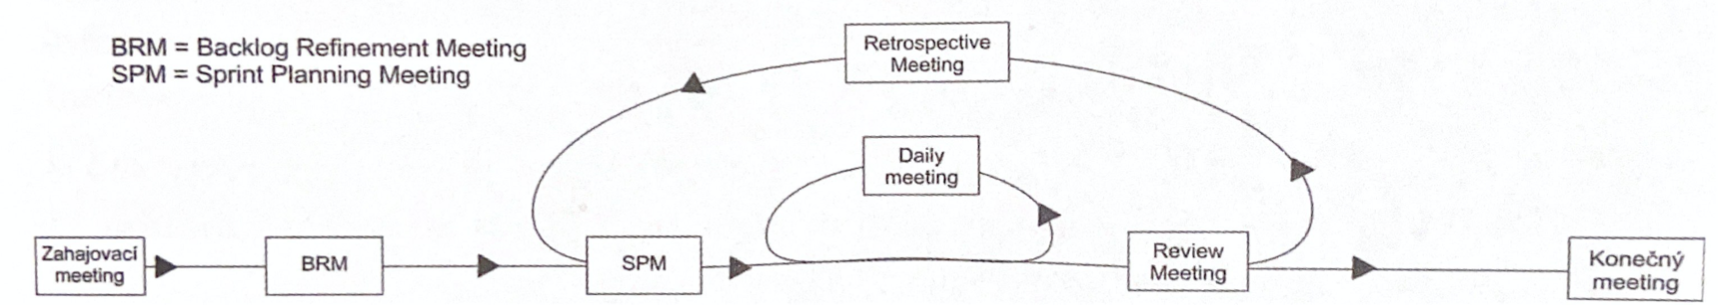
\includegraphics[width=1\textwidth]{Diplomka/Figures/scrum.png}
    \caption{Vývojový cyklus řízený pomocí metodiky Scrum (převzato z \cite{ref:scrum_myslin_cyklus_img})}
    \label{fig:scrum_cyklus}
\end{figure}

Jednotlivé schůzky by se poté daly rozdělit do tří základních skupin:

\begin{itemize}
\item Plánovací -- tento typ schůzek předchází jakékoli aktivitě, která po schůzce probíhá. Během těchto schůzek může být plánován buď celý projekt nebo naplánován sprint.
\item Hodnotící -- tyto schůzky probíhají buď na konci sprintu, nebo na konci projektu. Během tohoto typu schůzek se hodnotí, zda to co proběhlo, proběhlo v pořádku a případně, co bylo špatně. 
\item Plánovací i hodnotící -- do této skupiny spadá pouze denní schůzka zvaná \textit{Standup}. Během schůzky se jednak hodnotí předchozí den a plánuje se co se bude dále daný den dělat. Během schůzky mají všichni členové týmu možnost vidět, jak se úkol hýbe, nebo nehýbe.
\end{itemize}


Jednotlivé zadání úkolů jsou psány pomocí uživatelských příběhů (takzvané \textit{User stories}), přičemž většinou obsahují jen minimum technických informací. Jednotlivé uživatelské příběhy nepopisují interakci ze systémem. Uživatelské příběhy mají  sjednocenou podobu například ve tvaru: \uv{Jako \textit{role} chci \textit{cíl} tak, aby \textit{užitek}.} Tedy například: \uv{Jako uživatel chci vidět seznam zboží v objednávce, tak aby si uživatel mohl zboží zkontrolovat.} \cite{ref:scrum_myslin_us}

\subsection{V-Model}
V-model je grafické znázornění vývojového cyklu prakticky jakéhokoliv vývoje u kterého je důležité nepřetržité fungování a bezchybnost systému. Model je tedy využíván prakticky v každém odvětví, nejen v automobilovém průmyslu nebo softwarovém vývoji kritických systémů. Tento model zdědil po vodopádovém modelu jistou kaskádovitost, kdy každý krok je proveden až po předchozím kroku. Za rozdílnost V-Modelu lze považovat to, že je oproti agilním přístupům zaměřen na velmi důkladnou kontrolu a testování systému. Kontrola a testování probíhá již v počátečních etapách návrhu systému. Jednotlivé testování systému se provádí ve stejné době jako určitá část vývoje. Tedy například jednotkové testy se píšou během implementační části nebo například integrační testování probíhá při integraci jednotlivých komponent systému. Je vhodný zejména pro projekty, kde je většina požadavků jasná a předem daná. Grafické znázornění V-Modelu je možné vidět na obrázku \ref{fig:v_model}.

V-Model je graficky definován do tvaru velkého písmene V. Na levé straně modelu se nachází fáze spojené s verifikací. První fází v rámci verifikační části je sběr požadavků, ve kterém jsou od zákazníka získány požadavky. Tyto požadavky jsou následně analyzovány. V další fázi se provede na základě těchto nasbíraných požadavků návrh systému. Dále následuje vytvoření architektury systému a návrh jednotlivých modulů. Poté je na základě veškeré analýzy provedena implementace.

Na pravé straně jsou fáze validační, ve kterých se produkt testuje a validuje jeho funkčnost. Jednotlivé fáze jsou vzájemně propojené. Na nejnižší vrstvě probíhá jednotkové testování, které testuje chování malých modulů. Dále probíhá integrační testování, které je prováděno proti návrhu architektury. Jakmile je úspěšně provedeno integrační testování, tak je testován návrh systému systémovými testy. Na nejvyšší úrovní probíhá akceptační testování, které ověřuje, zda jsou správně naimplementovány veškeré definované požadavky zákazníka. Každý přechod do jiné fáze probíhá jakmile je kompletně splněna předchozí fáze.

 \begin{figure}[!ht]
    \centering
    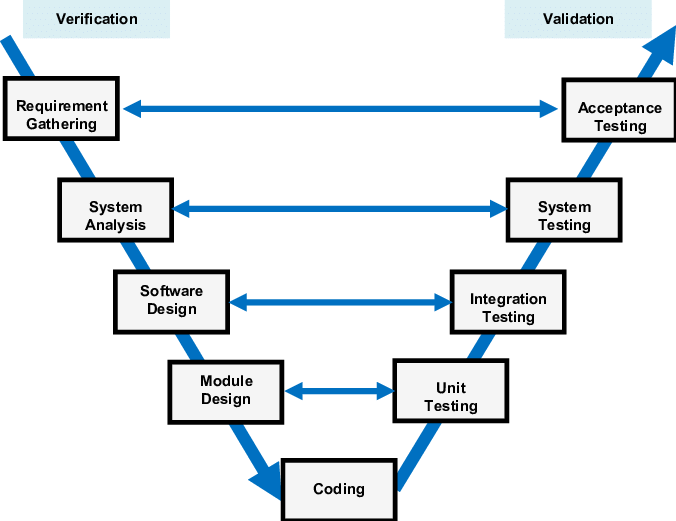
\includegraphics[width=0.7\textwidth]{Diplomka/Figures/v-model-in-software-testing.png}
    \caption{Grafické znázornění V-Modelu (převzato z \cite{ref:vmodel_Tierno2016})}
    \label{fig:v_model}
\end{figure}


\section{Metriky}
\label{sec:metrics}
Jelikož v rámci praktické části vytvářím nástroj pro metriky, je nutné se nejprve seznámit se samotnou teorií metrik a měření vývoje. Metriky se můžou používat nejen při samotném sběru požadavků, ale i při vývoji systému. Během sběru požadavků a vývoje celého systému je potřeba dodržovat určité standardy. V automobilovém průmyslu je to nejčastěji standard Automotive SPICE, který je podrobněji popsán v kapitole \ref{sec:aspice}. Pro to, aby bylo zajištěno plnění definovaného standardu a plnění jednotlivých úkolů pro dokončení projektu je využíváno právě metrik.

Dle výkladu Iana Sommervilla \cite{ref:metric_definition} je metrika softwaru vlastnost softwarového systému, systémové dokumentace nebo vývojového procesu , kterou lze objektivně měřit. Mezi typické obecné metriky můžeme zařadit například počet řádků kódu, počet splněných požadavků z celkového počtu zadaných, počet nalezených chyb v softwaru a další. Management mohou ovlivnit jak kontrolní, tak i prediktivní metriky. Při změně provedené na základě kontrolní metriky je změněn samotný softwarový proces. Pokud manažer provede rozhodnutí pro změnu v procesu mohou prediktivní metriky usnadnit odhad, jak bude změna náročná pro provedení změn. 

Při měření vývoje softwaru pomocí metrik se snažíme odvodit numerické hodnoty nebo profil atributu vývoje daného softwaru, části systému nebo dokonce i samotného procesu. Na základě naměřených údajů pomocí metrik dokážeme zjistit, jak je standard dodržován nebo jakým směrem se vývoj vyvíjí. Dále na základě těchto údajů dokážeme také zjistit kvalitu vyvíjeného systému nebo softwaru a také dokážeme hodnotit efektivitu jednotlivých procesů, které se při vývoji používají. Pomocí metrik také můžeme zjistit, zda používané nástroje a metody přispívají k lepší efektivitě či nikoliv.

Při zavádění nového nástroje v rámci organizace můžeme využít metriky tak, že část daného vývoje změříme metrikami před zavedení nástroje. Po určité definované době od zavedení nástroje pomocí metrik změříme znova stejnou část vývojového procesu a vyhodnotíme, zda je tým při vývoji efektivnější než před prvním měřením. Pod tímto si můžeme například představit zavedení nového nástroje na automatické testování vyvíjeného softwaru. Před zavedením pomocí metrik zjistíme, kolik se v softwaru vyskytuje chyb a poté tyto údaje porovnáme s údaji naměřenými po zavedení nástroje. Takto získaná data můžeme tedy používat pro zlepšení samotného vývoje a procesů.

Jedním ze základních dělení metrik je dělení na kontrolní a prediktivní metriky. Kontrolní metriky, jak již vyplývá ze samotného názvu, slouží pro správu a kontrolu prováděných procesů. Typické metriky patřící mezi kontrolní metriky je počet nahlášených chyb během vývoje, průměrný čas strávený na opravě detekovaných chyb, počet splněných úkolů od zahájení vývoje a mnoho dalších. Mezi prediktivní metriky řadíme metriky, které předpovídají vlastnosti vyvíjeného produktu nebo softwaru. Typickými představiteli je například cyklomatická složitost určité komponenty, počet tříd nebo databázových tabulek. Prediktivní metriky, které souvisejí s vlastnostmi vyvíjeného produktu nebo softwaru se mohou označovat také jako produktové metriky. \cite{ref:metric_definition} 

\subsection{Kontrolní metriky}
Tyto metriky slouží jako statistické údaje pro kontrolu daného softwarového procesu. Můžeme zde zařadit údaje stráveném času na nějakém konkrétním úkolu. Vysledovaná a naměřená data poté slouží jako podklad ke zlepšování osobního a softwarového procesu. 

Podle Iana Sommervilla \cite{ref:kontrolni_metriky} lze shromažďovat tři typy kontrolních metrik:

\begin{enumerate}
\item \textit{Zbývající čas, který je potřebný k dokončení definovaného procesu} -- v rámci této kategorie můžeme zařadit měření zbývajícího času k dokončení procesu, čas strávený testováním systému a další. V rámci této kategorie dokážeme určit efektivitu daného procesu. Z naměřených hodnot tedy dokážeme zjistit, zda se efektivita zvýšila nebo snížila.

\item \textit{Prostředky, které jsou nutné pro dokončení definovaného procesu} -- můžeme měřit například počet programátorů k dokončení určitého procesu, náklady spojené s vývojem systému a další. V této kategorii také dokážeme měřit efektivitu procesu například zda potřebné zdroje k dosažení výsledku klesají či nikoliv.

\item \textit{Počet zjištěných výskytů definované události} -- měříme a monitorujeme počet určitých vzniklých událostí, které můžou přímo nebo nepřímo ovlivňovat určitý proces. Můžeme zde uvést například počet nalezených chyb při testování, počet změněných požadavků, počet řádků kódu pro jeden požadavek a mnoho dalšího.

\end{enumerate}

V rámci kontrolních metrik můžeme tedy zjistit efektivitu samotného vývoje a lépe odhadnout směr vývoje procesu. Pomocí metrik můžeme měřit potřebný čas a úsilí k dokončení nebo posunu procesu. Například pomocí monitorování počtu vad dokážeme odhadnout kvalitu výsledného systému. Tedy při zvýšení počtu vad můžeme předpokládat, že v systému bylo nalezeno většiny chyb a systém bude tedy v produkčním prostředí stabilní a kvalitní. Je důležité zjistit, které informace je nutné pro následné zlepšení procesu a také systému sledovat, měřit a také shromažďovat.

\subsection{Prediktivní metriky}
Jak již bylo zmíněno, jde o metriky, které předpovídají vlastnosti výsledného produktu. Mezi prediktivní metriky můžeme zařadit produktové metriky, pomocí kterých dokážeme měřit interní atributy vyvíjeného produktu případně softwaru. Interní atributy si můžeme například představit jako konkrétní vlastnosti vyvíjeného softwaru. Jde tedy o velikost softwaru, počet naprogramovaných tříd, počet uživatelských obrazovek a mnoho dalšího. Tyto vlastnosti nemusí mít přímou spojitost na zjištění kvality softwaru, ale mohou sloužit jen jako informativní hodnota pro manažery pro odhad velikosti.

Produktové metriky lze dále dělit na dvě základní třídy podle původu měření. První třídou jsou statické metriky, které získávají data pomocí měření reprezentace systému -- dokumentace systému, návrh systému a samotný program. Můžeme zde zařadit počet tříd, počet formulářů, průměrná délka tříd a další. Tyto metriky nám dokáží usnadnit hodnocení a odhad složitosti a komplexnosti celého softwaru. Zároveň nám můžou být tyto informace užitečné pro přípravu na následnou údržbu celého systému.

Druhou třídou produktových metrik jsou dynamické metriky, pro která se data shromažďují průběžně pomocí spuštěného systému při testování nebo na produkčním prostředí. Tyto metriky nám pomáhají hodnotit celkovou spolehlivost systému v produkčním prostředí. Dále z těchto metrik můžeme odhadnout či zjistit náročnost a efektivitu systému pro produkční prostředí. Mezi dynamické metriky řadíme metriky měřící počet nedodělaných scénářů objevených testováním, počet nefunkčních požadavků nebo i informace o maximálním možné zatížení systému.

\subsection{Reprezentace a vizualizace metrik}
Metriku si můžeme představit jako sled čísel, které nám slouží jako ukazatele stavu procesu. Metriky můžeme tedy reprezentovat tak, abychom dokázali určit stav daného procesu nebo vyvíjeného systému. Pomocí metriky se může manažer rozhodovat o krocích, které budou podniknuty, aby byl proces efektivní a systém vytvořen v definované kvalitě a času. Nejčastěji si metriku můžeme představit jako tabulku a nebo pomocí grafické vizualizace, která vychází z dat tabulky.




% Bude napsáno o tom jak můžou metriky vypadat (tabulka, graf, ...) a jak je lze vizualizovat (birt + odkaz na praktickou část).

\subsubsection{Zobrazení pomocí tabulky}
Každou metriku si můžeme představit jako tabulku nasbíraných dat během procesu. Je to tedy základní vizualizace nasbíraných surových dat. Nevýhodou tabulkového zobrazení je, že při některých metrikách je složité a náročné si představit, co daná čísla reprezentují a zda číslo, které vidíme je dobré nebo špatné. Většinou se proto zobrazení tabulky kombinuje s grafem, pomocí kterého můžeme lépe pochopit daný kontext měřené veličiny.

\subsubsection{Vizualizace grafem}
Vizualizace pomocí grafu bývá jedna z nejčastějších možností, jak metriku zobrazit a následně pochopit. Pro kýženou vizualizaci grafem můžeme použít několik typů grafů. Vizualizace většinou vychází buď přímo ze surových dat nebo z připravených dat používaných pro zobrazení v tabulce. Pro vizualizaci dat je možné použít z několika stovek různých frameworků, které graf vytvoří a vizualizují. Mezi nejčastěji používané grafy patří různé variace sloupcového, spojnicového a koláčového grafu. V rámci IBM Jazz a aplikacích, které jsou naprogramované pomocí jazyka Java můžeme nalézt použitý framewrok BIRT, kterému se věnuji v rámci kapitoly \ref{sec:birt}. Druhou možností vizualizací na webových stránkách je pomocí JavaScriptové knihovny. V rámci této práce porovnávám dvě knihovny s názvem Google Charts a amCharts v kapitolách \ref{sec:google_charts} a \ref{sec:amcharts}.

\subsubsection{BIRT}
\label{sec:birt}
BIRT je open source softwarový projekt vyvíjený konsorciem Eclipse Foundation a původně sponzorovaná společností Actuate s pomocí společnosti IBM, který poskytuje platformu pro vytváření vizualizací dat. Je určený zejména pro webové a klientské aplikace, které jsou založených na prostředí Java a Java EE. BIRT se skládá ze dvou hlavních komponent \cite{ref:birt_about}:

\begin{itemize}
\item vizuální návrhář sestav v IDE Eclipse,
\item komponenta pro generování navržených sestav, které lze nasadit do libovolného Java prostředí.
\end{itemize}

Projekt BIRT také obsahuje mapovací modul, který je plně integrován do návrháře sestav a může být použit samostatně k integraci grafů do aplikace. Pomocí technologie BIRT je výstupy možné generovat kromě grafů ve formátu SVG, také jako seznamy dat (například pomocí tabulky) nebo jako textové dokumenty. Sestavy BIRT se skládají ze čtyř hlavních částí \cite{ref:birt_about}: 

\begin{itemize}
\item \textit{Data} -- poskytuje podporu pro přístup k datům pomocí JDBC, XML, webových služeb prostých databázových souborů. Vytvořená sestava může dále zobrazovat data z libovolného počtu zdrojů dat. BIRT využívá ODA (Open Data Access), který umožňuje komukoli vytvořit novou sestavu pro jakýkoli druh tabulkových dat.
\item \textit{Transformace dat} -- vygenerované reporty reprezentují shrnutá, seřazená, filtrovaná a seskupená data podle definovaných potřeb uživatele. Tato data jsou poté připravena pro vizualizaci.
\item \textit{Obchodní logika} -- jelikož jsou data v reálném světě málokdy strukturovaná přesně tak, aby vyhovovaly z byznysového hlediska pro jednotlivé reporty, je nutné je nejprve strukturovat tak, aby pro transformaci a vizualizaci vyhovovala. Tato strukturalizace je možná buď přímo pomocí BIRT v jazyku JavaScript, nebo externě pomocí zdrojového kódu v programovacím jazyku Java.

\item \textit{Vizualizace} -- Jakmile jsou data pro vizualizaci připraveny je možné je vizualizovat například pomocí grafů nebo tabulek. Jedna připravená sada dat může být vizualizována více způsoby.
\end{itemize}

Architektura BIRT se skládá z \textit{Report Designeru}, který zajišťuje vytváření reportů, které vygeneruje do formátu XML. Dále se skládá z \textit{Report enginu}, který vygeneruje jednotlivé vizualizace dat do definovaných formátů, jako například PDF, HTML, Excel, Word a další. Celkovou architekturu systému BIRT je možné vidět na obrázku \ref{fig:birtarch}.

\begin{figure}[!ht]
    \centering
    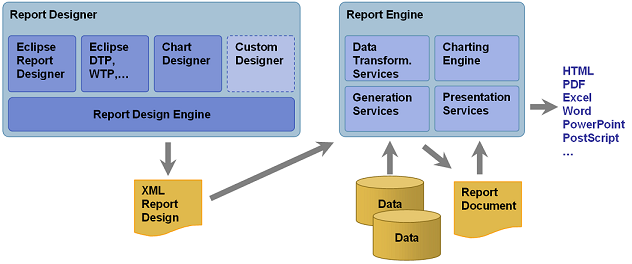
\includegraphics[width=0.8\textwidth]{Diplomka/Figures/birtarch.png}
    \caption{Architektura BIRT (převzato z \cite{ref:birt_about})}
    \label{fig:birtarch}
\end{figure}
\subsubsection{Metabase}
Podobně jako BIRT je Metabase možné použít jako nástroj pro zobrazování a vizualizaci neagregovaných dat. Je to moderní aplikace, kterou je možné spustit pomocí virtualizace Docker. Grafy je možné vytvářet a skládat pomocí SQL dotazů. Aplikace je poskytovaná jak zdarma, tak i za poplatek v případě hostování v cloudu nebo jako \textit{Enterprise} licence pro velké společnosti. Aplikaci je také možné použít jako celý \textit{Business intelligence}. Metabase je možné napojit na velké množství typů databází včetně MySQL, MongoDB, Oracle a další. Výstupní zprávy dokáže posílat také pomocí zpráv v aplikaci Slack. Není to tedy pouze knihovna sloužící pro vykreslení grafů, ale kompletní řešení. \cite{ref:metabase}


\subsubsection{Google Charts}
\label{sec:google_charts}
Je to veřejně dostupná interaktivní webová služba, která dokáže vytvořit grafy z poskytnutých dat. Knihovna je vyvinutá společností Google a je plně bezplatná.  Velkou výhodou knihovny je, že je plně přizpůsobitelná a funguje pomocí HTML5 a SVG. Zobrazení grafů je tedy kompatibilní na všech zařízení včetně mobilních telefonů a tabletů. Další výhodou je velká variace různých typů grafů, které mohou být zobrazovány dynamicky a při zobrazení měněny a lehce upravovány. Velkou nevýhodou je, že grafy nejsou plně interaktivní a není možné je za běhu bez nutnosti obnovení stránky měnit a jednoduše filtrovat. Oproti BIRT (viz kapitola \ref{sec:birt}) knihovna poskytuje pouze vizualizaci poskytnutých agregovaných dat.

Služba funguje jako JavaScriptová knihovna. Uživatel tedy dodá data pro JavaScript, který potřebný graf následně vykreslí. Služba vychází z původní Google Chart API, která fungovala čistě pomocí HTTP metod a není kompatibilní s aktuálním Google Charts. \cite{ref:google_charts}

\subsubsection{amCharts}
\label{sec:amcharts}
Je to jedna z mnoha knihoven fungujících na jazyku JavaScript pro vykreslování grafů na webových stránkách. Samotná knihovna je vytvořena v jazyku TypeScript. Vykreslování probíhá pomocí dynamického zobrazování SVG obrázků, které jsou plně kompatibilní jak s ovládáním pomocí myši, tak pomocí dotyků na mobilních zařízeních. Knihovna nepoužívá žádné jiné knihovny třetích stran a podporuje konfiguraci jak pomocí objektů v TypeScriptu nebo JavaScriptu, tak pomocí univerzálního JSONu. Knihovna obahuje obrovské množství různých typů grafů a jejich variací. Kromě klasických grafů nabízí také mapy, rozmanité diagramy a další variace různých typů grafů. Jednotlivé grafy je možné jakkoliv upravovat dle vlastního uvážení včetně typů písem a dalších vlastností. Grafy v amCharts vypadají moderně a obsahují mnoho volitelných animací a různě barevné šablony.  V základu také nabízí manipulaci s daty, které je možné skrývat či zobrazovat. Knihovna je v základní verzi se zobrazením loga v rohu každého grafu zdarma, pro odstranění loga je nutné zaplatit licenci. Podobně jako u služby Google Charts je nutné dodat data již připravené a agregované. \cite{ref:amcharts_web}

\subsubsection{Chart.js}
Chart.js je jednoduchá knihovna určená pro zobrazování grafů na webových stránkách. Knihovnu je možné získat plně zdarma a je dostupná jako otevřený software. Nabízí osm typů grafů, které mohou být animované a přizpůsobitelné. Grafy jsou generovány pomocí HTML5 Canvas a jsou tedy dostupné ve všech novějších prohlížečích. Komponenta je plně responzivní a je tedy možné ji použít na všechna možná zařízení. Nevýhodou je až moc velká jednoduchost a omezenost, která je však vykoupena rychlým nasazením do již existujících webových stránek. \cite{ref:chartjs}



\section{Automotive SPICE}
\label{sec:aspice}
Automotive Software Process Improvement and Capability Determination (zkráceně ASPICE) je standard, používaný v automobilovém průmyslu pro vývoj mechatronických a softwarových systémů v automobilovém průmyslu. Vychází z obecného standardu SPICE (ISO/IEC 15504), který se věnuje obecnému vývoji softwaru. Od vytvoření v roce 2005 je Automotive SPICE oborovou variantou této normy. Standard je volně přístupný na webových stránkách v několika světových jazycích \cite{ref:aspice_download_obecne}. Poslední dostupná verze je verze 3.1 z roku 2017. Tato verze obsahuje opravu drobných jazykových chyb a vychází z verze 3.0 \cite{ref:aspice_download_verze}.

Standard Automotive SPICE byl vyvinut v rámci spolupráce evropských automobilových společností. Ty se spojily do sdružení Automotive Special Interest Group (SIG). Dále je standard aktualizován skupinou Quality Management Center in the German Association of Automotive Industry (VDA QMC). Standard je tímto sdružením pravidelně aktualizován a upravován, aby vyhovoval nejnovějším požadavkům. Mezi evropské automobilky spojené do sdružení SIG patří například:

\begin{itemize}
  \item BMW Group,
  \item Daimler AG,
  \item Jaguar,
  \item Volkswagen AG,
  \item Volvo Car Corporation a další.
\end{itemize}

V současné době se automobily skládají z velkého množství součástí. Automobily se již neskládají pouze z mechanických součástí. V poslední době roste množství používaného softwaru nejen při vývoji ale i v samotných automobilech. Většina softwaru v automobilu slouží také pro zajištění nejen bezpečnostních funkcí, ale také pro zajištění životně důležitých funkcí automobilu včetně brzd a samotného řízení. Nesmí se tedy stát, že software v automobilu selže a například zablokuje brzdy a způsobí havárii. Dodržování tohoto standardu je rozhodující kritérium při volbě dodavatelů dané automobilové společnosti, jelikož zajišťuje že dodavatel splňuje určité standardy vývoje.

V rámci vývoje v automobilovém průmyslu je většina systémů vyvíjena pomocí V-Modelu. Každá část  vývojového procesu musí mít definovány cíle. Aby bylo možné určit, zda jsou cíle splněny jsou používány metriky (viz kapitola \ref{sec:metrics}). 

\subsection{Referenční procesní model}
Je to jeden z procesních modelů v rámci standardu Automotive SPICE. 
Každý proces obsahuje kromě popisu také funkční cíle v daném prostředí a seznam výsledků a výstupů, které má proces dosáhnout.
%Každý proces  je popsán v podmínkách prohlášení o účelu. Prohlášení o účelu obsahuje jedinečné funkční cíle procesu při provádění v konkrétním prostředí. Ke každému prohlášení o účelu je přidružen seznam konkrétních výsledků jako seznam očekávaných pozitivních výsledků výkonu procesu.
%Each process is described in terms of a purpose statement. The purpose statement contains the unique functional objectives of the process when performed in a particular environment. For each purpose statement a list of specific outcomes is associated, as a list of expected positive results of the process performance.
\cite{ref:aspice_download_procesni_modely}


Referenční procesní model definuje několik procesů ve třech základních kategoriích:

\begin{itemize}

\item primární procesy,
\item podpůrné procesy,
\item organizační procesy.

\end{itemize}

Jednotlivé kategorie procesů a samotné procesy jsou detailně probrány v kapitole \ref{sec:aspice_processes} a je možné je graficky seskupené vidět na obrázku \ref{fig:prm}. 
\begin{figure}[!ht]
    \centering
    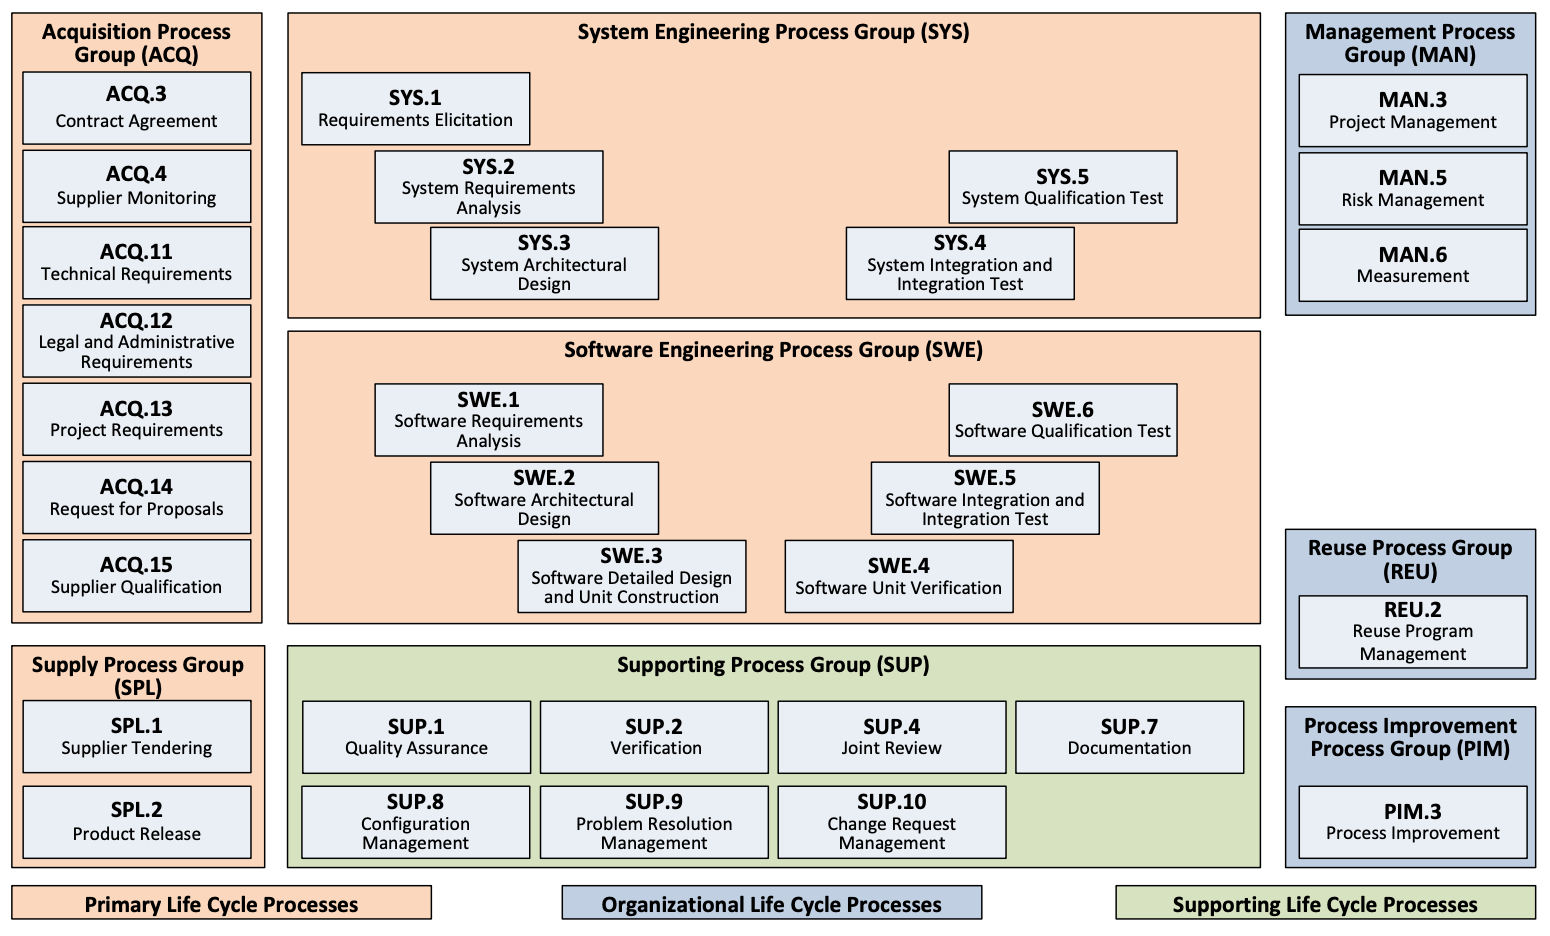
\includegraphics[width=1\textwidth]{Diplomka/Figures/prm.png}
    \caption{Referenční procesní model (převzato z \cite{ref:aspice_download_prm})}
    \label{fig:prm}
\end{figure}


% ) a je určen pro provádění hodnocení schopnosti používání tohoto softwarového procesu dodavatelem pro automobilový průmysl. 
% V rámci ASPICE existují dva druhy procesních modelů. První z nich je model hodnocení procesů (PAM), který byl vyvinut v souladu se standardem ISO/IEC 33004. Tento procesní model obsahuje několik hodnotících ukazatelů 

% PAM [3, str. 10] obsahuje sadu hodnotících ukazatelů výkonnosti a způsobilosti procesů. Tyto indikátory jsou základem pro shromažďování objektivních důkazů, které model umožňuje s posuzováním přiřadit hodnocení. Dále PAM definuje dvoudimenzionální model způsobilosti procesu. V první dimenzi proces jsou procesy definovány a rozděleny do kategorií procesů, kde v rámci kategorie procesů jsou procesy seskupeny do skupin procesů v druhém stupni v souladu se zabývanou druhou činností. V druhé dimenzi schopnost je definován soubor atributů procesu seskupených do úrovně schopností. Atributy procesu poskytují měřitelné vlastnosti způsobilosti procesu. Ještě dodáváme, že [4, str. 8] PAM poskytuje další ukazatele výkonnosti a způsobilosti procesů přizpůsobených potřebám k provádění posouzení softwarového procesu schopnosti dodavatelů pro automobilový průmysl. 



%Druhý procesní model je procesní referenční model (PRM). Ten se používá ve spojení s modelem hodnocení procesu při provádění hodnocení dané společnosti.
% \cite{ref:aspice_download_procesni_modely}

\subsection{Procesy Automotive SPICE}
\label{sec:aspice_processes}
V rámci každé základní kategorie procesů existují v referenčním procesním modelu podkategorie procesů, dle toho jakým okruhem činností se zaobírají. Procesy jsou pojmenovány pomocí třímístného identifikátoru, která určuje podkategorii procesu. Dále název procesu obsahuje číslo, které identifikuje proces v rámci své podkategorie.

\subsubsection{Primární procesy}
Kategorie primárních procesů životního cyklu sestává z procesů, které mohou být použity zákazníkem při získávání produktů od dodavatele, a dodavatelem při reakci a dodávce produktů zákazníkovi, včetně technických procesů potřebných pro specifikaci, návrh, vývoj, integraci a testování.

Mezi první podkategorii primárních procesů patří akviziční procesy. Do této podkategorie patří procesy, které jsou prováděny zákazníkem případně dodavatelem, který je v roli zákazníka, který požaduje  službu nebo produkt. Tato podkategorie akvizičních procesů obsahuje sedm procesů:

\begin{itemize}
	\item ACQ.3 -- Dohoda o smlouvě. Během tohoto procesu probíhá dohoda o samotné smlouvě a schválení smlouvy. Po úspěšném dokončení procesu je dohodnutá smlouva podepsaná a odsouhlasena všemi stranami.
	\item ACQ.4 -- Monitorování dodavatele. V průběhu procesu se monitoruje, zda dodavatel plní předem definované požadavky.
	\item ACQ.11 -- Technické požadavky. Jsou zde definovány technické požadavky, které je nutné plnit a kontrolovat. Do technických požadavků můžeme zařadit jak funkční, tak nefunkční požadavky na systém.
	\item ACQ.12 -- Právní a administrativní požadavky. V rámci tohoto procesu jsou řešeny veškeré právní závazky, definované jak ve smlouvě, tak i  na základě zákonů.
	\item ACQ.13 -- Požadavky na projekt. V průběhu procesu jsou definovány a ověřeny veškeré požadavky, které souvisejí s celým projektem. Můžeme zde zařadit například personální obsazení a další organizační aktivity.
	\item ACQ.14 -- Žádost o návrhy.  Během tohoto procesu jsou řešeny přípravy a vydání požadavků na daný systém.
	\item ACQ.15 -- Kvalifikace dodavatele. V tomto procesu jsou kontrolovány způsobilosti a kvalifikace dodavatele. V rámci procesu se ověřuje, zda dodavatel splňuje potřebné kvality pro výběrové řízení.
\end{itemize}

Dalším typem procesů jsou dodavatelské procesy. Tyto procesy jsou prováděny dodavatelem a výsledkem je dodání služby nebo produktu.

\begin{itemize}
	\item SPL.1 -- Výběrové řízení na dodavatele. Hlavní myšlenkou tohoto procesu je příprava a vytvoření nabídky do výběrového řízení.  Dále je v tomto procesu řešeno samotné podání nabídky do výběrového řízení.
	\item SPL.2 -- Vydání produktu. V rámci tohoto procesu se provádí předávání vyvinutého produktu zákazníkovi. Předávání produktu probíhá řízeně pomocí definovaných podprocesů. Během tohoto procesu se také vytváří předávací dokumentace. 
\end{itemize}	

Procesní skupina systémového inženýrství se skládá z procesů zaměřených na získávání a správu zákaznických a interních požadavků. Dále tyto procesy definují samotnou architekturu vyvíjeného systému. Procesy také řeší celkovou integraci systému a testování produktu na systémové úrovni.

\begin{itemize}
	\item SYS.1 -- Získání požadavků. Během procesu jsou požadavky nejen od zákazníka získány a zadefinování do projektu. Řadíme zde i další požadavky, jako jsou například interní a systémové. 
	\item SYS.2 -- Analýza systémových požadavků. V rámci tohoto procesu probíhá samotná analýza již nadefinovaných požadavků v předešlém procesu.
	\item SYS.3 -- Návrh architektury systému. Dochází k navrhnutí a vytvoření systémové architektury na základě definovaných požadavků na celý systém.
	\item SYS.4 -- Systémová integrace a testování integrace. Během procesu se provádí integrace jednotlivých částí systému a následné testování provedené integrace. Výsledkem procesu je otestovaný a zintegrovaný systém.
	\item SYS.5 -- Testování kvalifikace systému. V rámci procesu je provedeno otestování a schválení, zda výsledný systém splňuje všechny systémové požadavky. Výsledkem procesu je schválený systém, který je nachystaný pro samotné předání zákazníkovi.
\end{itemize}

Mezi poslední typ procesů primárních procesů patří procesy softwarového inženýrství. Tyto procesy se starají o správu softwarových požadavků, mezi které například patří například analýza softwarových požadavků, softwarová architektura a další.

\begin{itemize}
	\item SWE.1 -- Analýza softwarových požadavků, Během tohoto procesu dochází k analýze veškerých softwarových požadavků na systém, které vznikají ze systémových požadavků.
	\item SWE.2 -- Softwarový architektonický návrh. V procesu dochází k vytvoření architektonického návrhu. Dále se během procesu určí, které požadavky z procesu \textit{SWE.1} patří k jednotlivým částem systému. 
	\item SWE.3 -- Podrobný návrh softwaru a konstrukce jednotky. V rámci procesu je vytvořen podrobný návrh systémových komponent a jednotek.
	\item SWE.4 -- Ověření softwarových jednotek. Během procesu dochází k verifikaci navržených softwarových jednotek. Toto ověření probíhá na základě porovnání s funkčními a nefunkčními požadavky na systém.
	\item SWE.5 -- Integrace softwaru a test integrace. Dochází zejména k integraci navržených softwarových jednotek do celého systému, který je poté zevrubně kompletně otestován. 
	\item SWE.6 -- Kvalifikační testy softwaru. Během procesu je prováděno kvalifikační testování celého integrovaného systému ve shodě se všemi požadavky.
\end{itemize}

% \paragraph{Test Modified Paragraph}

\subsubsection{Podpůrné procesy}
Procesy zařazené v rámci sekce podpůrných procesů jsou použity v kterémkoli procesu v různých bodech celého vývojového životního cyklu. Procesy v této kategorii mají zkratku SUP.

\begin{itemize}
	\item SUP.1 -- Zajištění kvality. Proces zajišťuje, že veškeré používané procesy a pracovní nástroje splňují předem stanovené plány a potřebné kvality.
	\item SUP.2 -- Ověření. Proces je také nazýván verifikace a zajišťuje, že všechny pracovní nástroje a procesy splňují to co je požadováno.
	\item SUP.4 -- Společná kontrola. V rámci procesu probíhá společná kontrola a revize mezi všemi stranami, které se na projektu podílí. Je tedy zajištěno, že všechny strany vývoj systému a následný výsledek uspokojuje.
	\item SUP.7 -- Dokumentace. Během procesu je vytvářená důležitá dokumentace všech informací vzniklých během procesů.
	\item SUP.8 -- Správa konfigurace. Proces zajišťuje vytváření a údržbu všech pracovních nástrojů a produktů procesů nebo daného projektu.
	\item SUP.9 -- Správa řešení problémů. Veškeré problémy vzniklé během celého vývoje systému musí být identifikované a poté analyzované. V rámci procesu se poté také pracuje se samotnou správou a vyřešení problémů. 
	\item SUP.10 -- Správa požadavků na změnu. Dodržení procesu zajišťuje, že veškeré změny, které jsou navrženy jsou řízeny a sledovány.
\end{itemize}

\subsubsection{Organizační procesy}
Poslední skupinou v rámci Automotive SPICE jsou organizační procesy, které se zaměřují na produktové, procesní a zdrojové aktiva. Ta pokud jsou používaná v rámci projektů dané společnosti, pomohou v dosahování obchodních cílů.

Skupina procesů řízení se skládá z procesů, které může použít kdokoli, kdo v rámci vývojového životního cyklu řídí jakýkoli typ projektu nebo procesu. Tato skupina procesů má zkratku MAN.

\begin{itemize}
	\item MAN.3 -- Projektový management. Proces zahrnuje celé projektové řízení a je důležitý pro nalezení aktivit a nutné zdroje k vytvoření celého systému.
	\item MAN.5 -- Řízení rizik. Veškeré rizika spojené s vývojem systému musí být identifikovány a poté řízeny, tak aby nedošlo k problémům.
	\item MAN.6 -- Měření. V rámci procesu jsou měřeny a sbírány data týkající se celého vývoje. Na základě naměřených dat můžeme zajistit lepší a efektivnější směrování celého projektu. Dále měřením můžeme reflektovat určitou kvalitu celého nebo části systému.
\end{itemize}

Další skupinou v rámci organizačních procesů je skupina vylepšení procesů se zkratkou PIM. V této skupině existuje jeden proces. Tento proces obsahuje postupy pro zlepšení jednotlivých procesů prováděných v rámci společnosti.

\begin{itemize}
	\item PIM.3 -- Vylepšení procesu. Proces je velmi důležitý pro zajištění neustálého zlepšování efektivity při vykonávání všech ostatních procesů v rámci celé společnosti vyvíjející daný systém. Proces nám zajistí, že veškeré procesy jsou efektivní a vyhovující.
\end{itemize}

Poslední skupinou organizačních procesů je skupina procesu opětovného použití. Tato skupina má zkratku REU a obsahuje pouze jeden proces. Tento proces slouží k zavádění opětovného použití procesů v rámci společnosti.

\begin{itemize}
	\item REU.2 -- Opětovné použití správy programu. Během procesu je zajištěna celá správa znovupoužití programu v celé společnosti vyvíjející daný systém. Důležité je zajistit, že použitý program je využíván systematicky a efektivně.
\end{itemize}


Kompletní znění a definice všech jednotlivých procesů je možné nalézt v standardu Automotive SPICE. \cite{ref:aspice_procesy} Ve standardu se dále vyskytují také podmínky pro úspěšné splnění a použití daných procesů.


\subsection{Hodnotící framework}
Hodnotící framework poskytuje nezbytné požadavky a pravidla pro zjištění jakým způsobem se dané procesy v rámci projektu používají. Poskytuje schéma a návod, které umožňuje hodnotiteli určit úroveň schopnosti procesu, který daná firma u projektu používá. Tyto úrovně jsou definovány v rámci hodnotícího frameworku pomocí procesních atributů. Jednotlivým úrovním se věnuji v následujících kapitolách. Dané procesní atributy jsou přiřazené jednotlivým úrovním. Míra dosažení určitého procesního atributu je reprezentována pomocí hodnocení na základě definované hodnotící stupnice. Konečnou úroveň rozhodne na základě pravidel hodnotitel. Pravidla jsou reprezentována jako atributy které musí daný proces obsahovat. Automotive SPICE pro toto používá standard ISO/IEC 33020. \cite{ref:aspice_download_1523}

\subsubsection{Úrovně způsobilosti procesu a atributy procesu}
Jak již bylo zmíněno v předchozí kapitole, Automotive SPICE používá pro úrovně způsobilosti standard ISO/IEC 3302. Procesní atributy jsou vlastnosti procesu, které lze hodnotit na stupnici 0 až 5 a poskytují měřítko schopnosti procesu. Úrovně způsobilosti jsou použitelné pro všechny druhy procesů. Jednotlivé dodržení úrovně způsobilosti hodnotí hodnotitel na základě dodržení definovaných procesních atributů pro každou úroveň. Každá vyšší úroveň zároveň obsahuje podmínku pro 100\% splnění předchozí úrovně.

\begin{itemize}
\item Úroveň 0: Neúplný proces -- proces na této úrovni není vůbec implementován a definován nebo nedosahuje cíle. Patří zde také procesy, které dodržují procesní atributy, které ASPICE definuje nejvýše na úroveň \textit{částečně dosaženo} (P) (viz kapitola \ref{sec:process_atributes}).

\item Úroveň 1: Vykonávaný proces -- implementovaný proces na této úrovni plní svůj procesní účel. Během procesu projde vývoj celým V modelem, ale budou v něm mezery a nedokonalosti. K dosažení této úrovně musí být splněn atribut PA 1.1 -- výkonnostní atribut procesu.

\item Úroveň 2: Řízený proces -- Vykonávaný proces je nyní implementován v řízeném prostředí. Proces je plánován, monitorován a uzpůsoben dle požadavků. Vyvinuté produkty jsou náležitě zavedeny, kontrolovány a udržovány. V rámci této úrovně musí být splněny procesní atributy PA 2.1 -- řízení výkonu a PA 2.2 - řízení pracovního produktu.

\item Úroveň 3: Zavedený proces -- Dříve popsaný řízený proces je nyní implementován pomocí definovaného procesu, který je schopen dosáhnout svých výsledků procesu. Společnost, která má proces na této úrovní má centralizované standardy, jak pracuje, a daný projekt se těmito standardy řídí. Na úrovni 3 je nutné splnit procesní atributy PA 3.1 -- definice procesu a
PA 3.2 -- procesní nasazení.

\item Úroveň 4: Předvídatelný proces -- Dříve popsaný zavedený proces nyní pracuje prediktivně v definovaných mezích, aby dosáhl svých procesních výsledků. Úroveň 4 zahrnuje procesní atributy PA 4.1 -- kvantitativní analýza a PA 4.2 -- kvantitativní kontrola.

\item Úroveň 5: Optimalizovaný proces -- Výše popsaný předvídatelný proces je nyní neustále vylepšován, aby reagoval na změny v dané společnosti. Pátá úroveň zahrnuje dva procesní atributy PA 5.1 -- inovace procesu a PA 5.2 -- implementace procesní inovace.

\end{itemize}

\subsubsection{Hodnocení procesních atributů}
\label{sec:process_atributes}
Aby mohl proškolený hodnotitel hodnotit úroveň způsobilosti procesu v určité společnosti, určuje Automotive SPICE hodnotící stupnici, která pochází ze standardu ISO/IEC 33020. Definované procesní atributy jsou hodnoceny na základě splnění podmínek, které určuje daný proces. Rozšířená stupnice pro hodnocení procesních je možné vidět v tabulce \ref{tab:aspice_rating_scale}.


\begin{table}[htp]
\begin{center}
\begin{tabular}{c | c | c | m{6cm}}

\multicolumn{2}{c|}{\textbf{Hodnocení}} & \multicolumn{1}{c|}{\textbf{Úroveň dosažení}} & \multicolumn{1}{c}{\textbf{Popis}} \\ 
\hline
\hline
%\vcell{N}  & \vcell{Nedosaženo} & \vcell{dosažení 0 \% až 15 \%} & \vcell{Existují jen malé nebo žádné důkazy o dosažení definovaného atributu procesu v posuzovaném procesu} \\ 
% \printcellmiddle & \printcellmiddle  & \printcellmiddle & \printcelltop \\
N  & Nedosaženo & dosažení 0 \% až 15 \% & V projektu existují malé nebo žádné důkazy o dosažení definovaných procesních atributů v posuzovaném procesu. \\ 
\hline
P- & Částečně nedosaženo & dosažení 15 \% až  32,5 \% & V rámci projektu existuje několik důkazů o dosažení procesního atributu v posuzovaném procesu. Mnoho aspektů k dosažení procesního atributu můžou být nepředvídatelné. \\ 
\hline
P+ & Částečně nedosaženo & dosažení  32,5 \% až 50 \% & V rámci projektu existuje několik důkazů o dosažení procesního atributu v posuzovaném procesu. Některé aspekty k dosažení procesního atributu můžou být nepředvídatelné. \\ 
\hline
L- & Téměř dosaženo & dosažení  50 \% až 67,5 \% & V projektu se systematicky přistupuje k  definovanému procesnímu atributu a jeho významném dosažení. V posuzovaném procesu může existovat mnoho slabin souvisejících s tímto procesním atributem. \\ 
\hline
L+ & Téměř dosaženo  & dosažení  67,5 \% až 85 \% & V projektu se systematicky přistupuje k definovanému procesnímu atributu a jeho významném dosažení. V posuzovaném procesu mohou existovat některé slabiny související s tímto procesním atributem. \\ 
\hline
F  & Plně dosaženo & dosažení  85 \% až 100 \% & V projektu se úplně a systematicky přistupuje k definovanému procesnímu atributu a jeho úplném dosažení v posuzovaném procesu. V posuzovaném procesu neexistují žádné významné slabiny související s tímto procesním atributem. \\ 
\end{tabular}
\caption{Rozšířená stupnice hodnocení procesu v ASPICE dle ISO/IEC 33020 \cite{ref:aspice_download_1523}}
\label{tab:aspice_rating_scale}
\end{center}
\end{table}

\subsubsection{Model úrovně způsobilosti procesu}
Úroveň způsobilosti procesu určí hodnotitel na základě hodnocení procesních atributů. Model definuje  pravidla, na základě kterých je úroveň určena. Proces může úrovně dosáhnout pouze pokud jsou procesní atributy dané úrovně ohodnoceny alespoň L (téměř dosaženo) a zároveň pokud jsou veškeré nižší úrovně procesních atributů splněny na F (plně dosaženo).


\subsection{Metriky a monitorování procesu}
Automotive SPICE klade velké nároky na kvalitní výsledky při vývoji a dodržování standardu. Proto jsou také v rámci standardu definovány procesy, které sledují dodržování kvality jiných procesů a podporují měření a monitorování samotného vývoje.



\section{Application Lifecycle Management}

Application Lifecycle Management není pouze proces samotného vývoje a programování softwaru. Je to možné přirovnat k životě člověka, kdy jde o kompletní proces, začínajíc od první myšlenky a požadavku zákazníka zákazníka, přes samotný vývoj softwaru a nasazení do produkčního prostředí. Application Lifecycle Management končí až jakmile končí samotný software, kdy například přestane dávat z byznysového hlediska smysl. \cite{alm_chappell}

Application Lifecycle Management je možné rozdělit na tři základní aspekty, které je možné vidět na obrázku \ref{fig:alm}:

\begin{itemize}
  \item řízení,
  \item vývoj,
  \item provoz.
\end{itemize}

\begin{figure}[!ht]
    \centering
    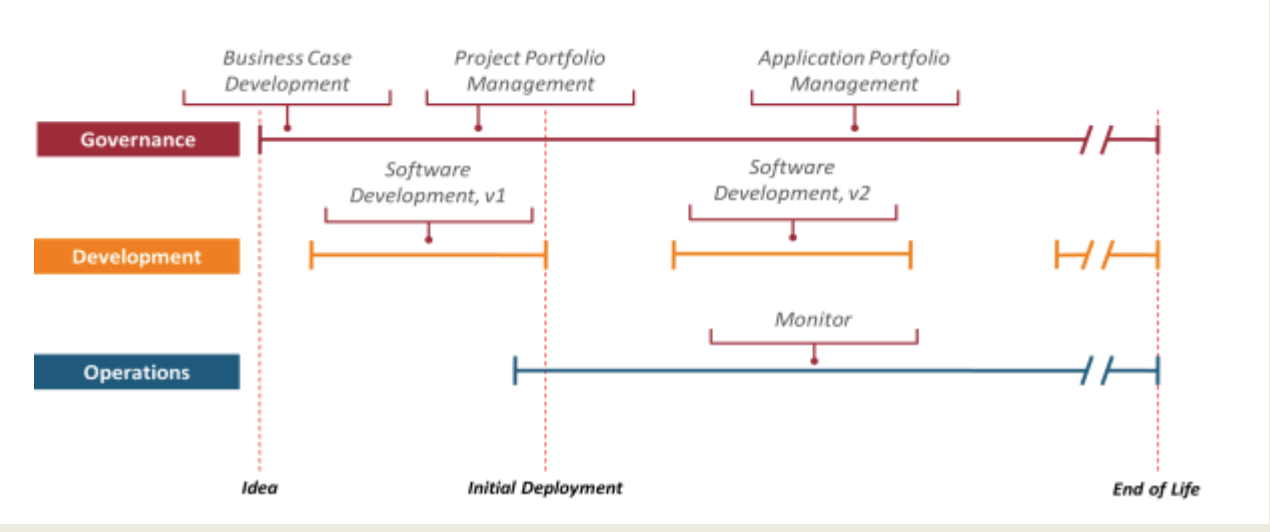
\includegraphics[width=1\textwidth]{Diplomka/Figures/alm.png}
    \caption{Aspkety ALM a jejich fáze \cite{alm_chappell}}
    \label{fig:alm}
\end{figure}

Proces, který probíhá během celého aplikačního cyklu je řízení. Vzniká počáteční myšlenkou zákazníka a pokračuje až do konce života softwaru. Během této činnosti jsou prováděny rozhodovací procesy, plánování, sběr požadavků a samotné řízení projektu. Je to nejdůležitější aspekt celého aplikačního cyklu. Pakliže by tento proces nebyl správně dodržován, nemusí být naplněna byznysová hodnota daného softwaru. \cite{alm_chappell} První fází, kterou proces začíná je \textit{Business Case Development}, ve kterém je řešen sběr požadavků zákazníka a vytvoření základní koncepce vývoje. Poté se v rámci fáze \textit{Project Portfolio Managmentu} řeší procesy spojené s organizací vývoje a nasazení do produkčního prostředí. V rámci poslední fáze, která probíhá po nasazení do produkčního prostředí má manažer na starosti kontrolovat, zda daný software splňuje požadavky zákazníka.

Proces vývoje začíná jakmile je sběr požadavků dokončen a funkčnosti jsou specifikované. Hlavní část procesu probíhá až do nasazení softwaru do produkčního prostředí. Po nasazení do produkčního prostředí vývoj probíhá již jen v menších fázích, ve kterých má zákazník další nové požadavky, které si přeje dodělat. Nové požadavky na funkčnost mohou vzniknout například proto, aby daný software ustál v konkurenčním prostředí. \cite{alm_chappell}. V rámci jednotlivých fázích vývoje tedy probíhá postupně nejprve základní první verze daného softwaru. Po nasazení do produkčního prostředí probíhá jednak údržba systému a také vývoj nových funkcionalit (viz Obrázek \ref{fig:alm}).

Samotný provoz softwaru začíná jakmile je vývoj dokončen. Provoz probíhá až do úplného ukončení činnosti softwaru. Během tohoto procesu probíhá práce spojené s během a udržováním aplikace. Během tohoto aspektu je software nasazován do produkčního prostředí a monitorován jeho běh.  \cite{alm_chappell} 

Každá část životního aplikačního cyklu se liší dle použitého vývojového procesu. Rozdílně vývoj probíhá při agilním procesu nebo při vodopádovém modelu. Jednotlivým vývojovým procesům se věnuji v rámci kapitoly \ref{sec:sw_process}.


% ALM aplikace se používají pro plánování a monitorování procesu. Na základě zmonitorovaných dat je poté proces upravován a měněn tak aby bylo možné produkt dokončit úspěšně za co nejmenších nákladů. Aplikací .

\subsection{codeBeamer}

\subsection{Siemens Polarion}

\subsection{IBM Jazz}

\subsubsection{Sběr požadavků}

\subsubsection{Monitorování procesů}

\subsubsection{Export dat}


\subsection{Porovnání aplikací}

\newpage % ODSTRANIT
\section{Business intelligence aplikace}


\subsection{Qlik}

\subsection{Microsoft Power BI}

\subsection{Porovnání aplikací}

\newpage % ODSTRANIT
\section{Vlastní aplikace}
TODO - praktická část.

Aplikace je realizována jako webová aplikace.

\subsection{Architektura a použité technologie}

\subsubsection{Symfony}

\subsubsection{MongoDB}

\subsubsection{MySQL}


\subsection{Import dat z IBM Jazz}
popsat jednotlivé druhy napojení na jazz, Automaticky pomocí cronu, rest api 

\subsection{Uložení dat}
Kontroly importů duplicitních, přidávání dat k importu, GUI práce nad daty, promazávání apod.

\subsection{Zpracování dat}
předpříprava dat query language

\subsection{Definice metrik}
report builder

\subsection{Zobrazení metrik}
pomocí js


\subsection{Výstupní reporty}
Pdf, excel. Definování vlastního reportu, automatické ukládáni na projekt atd.
    

\section{Závěr}
TODO 

\begin{thebibliography}{26}

\bibitem{ref:sommerrville_sw_process}
SOMMERVILLE, Ian. \textit{Software engineering}. 9th edition. Boston: Addison-Wesley, 2011, s.~28-29. ISBN 978-0-13-703515-1.

\bibitem{ref:sw_process_vondrak}
\textit{Úvod do softwarového inženýrství} [online]. In: VONDRÁK, Ivo. Ostrava, 2002, s. 3 [cit. 2020-11-30]. Dostupné z: http://vondrak.cs.vsb.cz/download/Uvod\_do\_softwaroveho\_inzenyrstvi.pdf

\bibitem{ref:cmm_cmmi}
Software measurement and metrics. SOMMERVILLE, Ian. \textit{Software engineering}. 9th edition. Boston: Addison-Wesley, 2011, s.~721-722. ISBN 978-0-13-703515-1.

\bibitem{ref:sommerrville_waterfall}
SOMMERVILLE, Ian. \textit{Software engineering}. 9th edition. Boston: Addison-Wesley, 2011, s.~29-32. ISBN 978-0-13-703515-1.

\bibitem{ref:rup_ibm_about}
\textit{Rational Unified Process: Best Practices for Software Development Teams} [online]. In: . Rev 11/01. Cupertino: Rational Software, 1998, s.~1 [cit. 2020-11-21]. Dostupné z: https://www.ibm.com/developerworks/rational/library/content/03July/
1000/1251/1251\_bestpractices\_TP026B.pdf

\bibitem{ref:rup_ibm}
\textit{Rational Unified Process: Best Practices for Software Development Teams} [online]. In: . Rev 11/01. Cupertino: Rational Software, 1998, s.~3 [cit. 2020-11-21]. Dostupné z: https://www.ibm.com/developerworks/rational/library/content/03July/
1000/1251/1251\_bestpractices\_TP026B.pdf

\bibitem{ref:agilne_manifesto}
\textit{Manifest Agilního vývoje software} [online]. 2001 [cit. 2020-11-21]. Dostupné z: https://agilemanifesto.org/iso/cs/manifesto.html

\bibitem{ref:sommerrville_agile_products}
SOMMERVILLE, Ian. \textit{Software engineering}. 9th edition. Boston: Addison-Wesley, 2011, s.~59. ISBN 978-0-13-703515-1.

\bibitem{ref:what_is_xp}
BECK, Kent a Cynthia ANDRES. \textit{Extrémní programování: embrace change}. 2nd ed. Praha: Grada, 2002, s.~1---7. Moderní programování. ISBN 80-247-0300-9.

\bibitem{ref:scrum_myslin}
MYSLÍN, Josef. \textit{Scrum: průvodce agilním vývojem softwaru}. Brno: Computer Press, 2016. ISBN 978-80-251-4650-7.

\bibitem{ref:scrum_myslin_cyklus_img}
MYSLÍN, Josef. \textit{Scrum: průvodce agilním vývojem softwaru}. Brno: Computer Press, 2016 s.~85. ISBN 978-80-251-4650-7.

\bibitem{ref:scrum_myslin_us}
MYSLÍN, Josef. \textit{Scrum: průvodce agilním vývojem softwaru}. Brno: Computer Press, 2016 s.~89. ISBN 978-80-251-4650-7.

\bibitem{ref:vmodel_Tierno2016}
TIERNO, Antonio, Max M. SANTOS, Benedito A. ARRUDA a Joao N. H. DA ROSA. Open issues for the automotive software testing. \textit{2016 12th IEEE International Conference on Industry Applications (INDUSCON)} [online]. IEEE, 2016, 2016, , 1-8 [cit. 2020-11-27]. ISBN 978-1-5090-5127-4. Dostupné z: doi:10.1109/INDUSCON.2016.7874609

\bibitem{ref:metric_definition}
Software measurement and metrics. SOMMERVILLE, Ian. \textit{Software engineering}. 9th edition. Boston: Addison-Wesley, 2011, s.~668. ISBN 978-0-13-703515-1.


\bibitem{ref:kontrolni_metriky}
Software measurement and metrics. SOMMERVILLE, Ian. \textit{Software engineering}. 9th edition. Boston: Addison-Wesley, 2011, s.~711-7114. ISBN 978-0-13-703515-1.

\bibitem{ref:birt_about}
BIRT Design Overview. \textit{BIRT} [online]. Ottawa: The Eclipse Foundation, 2014, 2014 [cit. 2020-11-28]. Dostupné z: https://www.eclipse.org/birt/about/

\bibitem{ref:metabase}
\textit{Metabase} [online]. San Francisco: Metabase, c2021 [cit. 2021-01-15]. Dostupné z: https://www.metabase.com/

\bibitem{ref:google_charts}
Charts | Google Developers. \textit{Google} [online]. [cit. 2021-01-08]. Dostupné z: https://developers.google.com/chart

\bibitem{ref:amcharts_web}
\textit{JavaScript Charts \& Maps - amCharts} [online]. amCharts, c2006-2021 [cit. 2021-01-15]. Dostupné z: https://www.amcharts.com/

\bibitem{ref:chartjs}
\textit{Chart.js | Open source HTML5 Charts for your website} [online]. https://www.chartjs.org/, c2021 [cit. 2021-01-15]. Dostupné z: https://www.chartjs.org/

\bibitem{ref:aspice_download_obecne}
Automotive SPICE | Download. \textit{Automotive SPICE} [online]. 2005, 2018 [cit. 2020-11-17]. Dostupné z: http://www.automotivespice.com/download/

\bibitem{ref:aspice_download_verze}
\textit{Automotive SPICE Process Reference and Assessment Model - Release 3.1} [online]. \textbf{1 November 2017}, s.~4 [cit. 2020-11-17]. Dostupné z: http://www.automotivespice.com/download/

\bibitem{ref:aspice_download_procesni_modely}
\textit{Automotive SPICE Process Reference and Assessment Model - Release 3.1} [online]. \textbf{1 November 2017}, s.~8 [cit. 2020-11-17]. Dostupné z: http://www.automotivespice.com/download/

\bibitem{ref:aspice_download_prm}
\textit{Automotive SPICE Process Reference and Assessment Model - Release 3.1} [online]. \textbf{1 November 2017}, s.~12-15 [cit. 2020-11-17]. Dostupné z: http://www.automotivespice.com/download/


\bibitem{ref:aspice_procesy}
\textit{Automotive SPICE Process Reference and Assessment Model - Release 3.1} [online]. \textbf{1 November 2017}, s.~13-15 [cit. 2021-01-01]. Dostupné z: http://www.automotivespice.com/download/

\bibitem{ref:aspice_download_1523}
\textit{Automotive SPICE Process Reference and Assessment Model - Release 3.1} [online]. \textbf{1 November 2017}, s.~15-23 [cit. 2020-11-18]. Dostupné z: http://www.automotivespice.com/download/

\bibitem{alm_chappell}
\textit{What is Application Lifecycle Management?} [online]. 2014, , 2-4 [cit. 2020-11-15]. Dostupné z: http://davidchappell.com/writing/white\_papers/What-is-ALM--Chappell.pdf


\end{thebibliography}

\end{document}
